%\documentclass{article}
\documentclass[12pt]{article}

%\usepackage{sbcstyle}


\usepackage{graphicx,subfigure} %package to manage images
\graphicspath{ {Figure/} }
\usepackage[rightcaption]{sidecap}
\usepackage{wrapfig}

%\usepackage[english]{babel}
\usepackage[utf8]{inputenc}
\usepackage{url}
\usepackage{graphicx}
% margem sup 3.5 cm: h� 1,5 cm para header, + 2 cm para top
% margem inf 2.5 cm: h� 1,5 cm para foot, + 1 cm para bottom
% margem esq/dir 3 cm
%\RequirePackage[a4paper,top=3.5cm,left=3cm,right=3cm,bottom=2.5cm]{geometry}

\RequirePackage[a4paper,top=2.5cm,left=2.5cm,right=2.5cm,bottom=2.5cm]{geometry}


\parindent 1.27cm
\parskip   6pt


\usepackage{array}
\usepackage{multirow}
\usepackage{tabu}
\usepackage{subfigure}
\usepackage[squaren,Gray]{SIunits}
\usepackage{tabularx}
\usepackage{colortbl}



\title{Etat de l'art}
\author{joel ortiz sosa }
\date{September 2016}

\usepackage{natbib}
\usepackage{graphicx}






\begin{document}

\maketitle

\section{Introduction}
The growing demand for faster devices with low energy consumption in different applications, such as: smart phones, mobile medical devices, IoT devices, automotive and aerospace, weather forecasting, astronomical data analysis and bioinformatics applications, it has evolved conventional architecture of a SoC (system on Chip). To increase the speed of data processing, formerly it was necessary to increase the frequency of operation but increase the frequency entailed an increase in energy consumption. To prevent the growth of energy consumption due to the frequency, the trend in microprocessor architecture design is to achieve better performance using parallelism\citep{2006}. Instead of using one processing core with higher frequency, more cores can be integrated on the same chip with the same total area (thanks to scaling down transistor dimensions), each operating at a reasonable frequency in terms of power consumption. 
But many-cores in a SoC creates a communication bottleneck, conventionally overcome by using the Network-On-Chip (NoC) paradigm as a scalable interconnection infrastructure for multi-core chips \citep{976921} overcoming the limitations of shared bus communication on SoCs. Today’s, several multi-core architectures which use a NoC as interconnection backbone, are already in the market \citep{2709201601}, \citep{2709201602}. The number of processing cores integrated into such architectures is currently in the order of hundreds and it is expected to exceed the thousands by around 2020 according to the international Technology Roadmap for semiconductors (ITRS).
Many advances in NoC research, including power efficiency, reliability and sustainability, have made it a valid choice as a communication backbone in multicore and many-core chips. However, according to the ITRS on-chip metal/dielectric based interconnect is the major bottleneck to overcoming the power-performance barrier in the future generations, because the ever more increasing number processing cores, makes the on-chip communication system the main responsible of the scalability limitations in terms of wiring delay, global synchronization and energy consumption. It is mainly due to the multi-hop nature of traditional wire-based NoC architectures in which the communication latency increase with the network size.
To face with this problem, several emerging communication architectures emerging communication such as 3D NoC \citep{6513612}, Optical, RF-I transmission lines, surface wave interconnects(SWI) and Wireless NoC (WiNoC) architectures have been proposed in literature  \citep{5071456}, \citep{7404347}. 3D NoC offers many advantages but also adds significant thermal constraints; the major drawback of optical NoC is the need of an external light source; the main challenge that faces the RF-I is crosstalk among TLs and between TLs and surrounding circuitry, especially at high frequency or in long TLs; SWI is considered to be one of the newest emerging interconnects. Hence, requires research to tackle a set of design and implementation challenges at different levels in order for it to be used in future NoC; however, WiNoC technology is considered to be the most mature emerging interconnect types since many implementations of WiNoC components such as integrated antennas and transceivers have been presented in the literature \citep{1459088}, \citep{5296159}, \citep{6569587}, \citep{7459514}. Wireless communication in NoCs enable one-hop data transfers between distant nodes and hence reduce the hop counts in inter-core communication. In addition to reducing interconnect delay, eliminating multi-hop long-distance wired communication reduces energy dissipation as well. But there is a price to pay in terms of silicon area due for transceivers and antennas. Such limitation is overcome by limiting the number of radio-hubs and by optimizing their topological mapping \citep{6302124}. However, there are some challenges facing WiNoC. For instance, researches are finding it difficult to design an antenna with wide frequency bandwidth, low power dissipation, larger coverage area and small area overhead \citep{6197727}.





\section{Physical layer design}

In a WiNoC, the miniaturized on-chip antennas and wireless transceivers influence the performance of the physical layer, mainly because the adopted frequency range of communication has an impact in the characteristics of the antennas and transceivers. Different research groups have classified WiNoC into for classes depending on their frequency range of operation: Ultra-Wide Band (UWB), Millimeter (mm)-Wave, Sub Terahertz (Sub-THz) and Terahertz. 

\subsection{Ultra-Wide Band (UWB)}

One possibility for WiNoC design is to use UWB intra-chip communication because it has a great performance in short distance, low transmit power and is a low-complexity radio technology. In the literature, we can find a UWB transceiver utilized for WiNoCs \citep {4531729} , developed in 90 nm. The transmitter counts with a CMOS integrated Gaussian monocycle pulse (GMP) to create an ultra-short pulse giving rise to extremely low power spectral density. The receiver consists of a wideband LNA, a correlator, an ADC and synchronization circuits. The antenna used is meander type dipole with 1 mm of data transmission range at antenna length of 2.98 mm. Its transceiver can sustain 1.16 Gb/s for a single channel at central frequency of 3.6 GHz. 


\subsection{Millimeter (mm)-Wave}
\subsection{Sub Terahertz (Sub-THz)}
\subsection{Terahertz}

\begin{table}[htb]
\centering
\caption{WiNoC physical layer characteristics}
\label{Table1}
\resizebox{16cm}{!} {
\begin{tabular}{|c|c|c|c|c|c|c|}
\hline
Frequency Range & Technology & Antenna Used & Modulation Scheme & Transmission Range & \begin{tabular}[c]{@{}c@{}}Data Rate\\ (Gbps)\end{tabular} & Energy per bit \\ \hline
\begin{tabular}[c]{@{}c@{}}UWB\\ (3 to 10 GHz)\end{tabular} & 90 nm & Meander type dipole & \begin{tabular}[c]{@{}c@{}}Pulse position\\ modulation (PPM) or \\ biphase modulation \\ (BPM)\end{tabular} & 1 mm & 1.16 & Not available \\ \hline
\begin{tabular}[c]{@{}c@{}}mm-Wave\\ (10 to 100 GHz)\end{tabular} & 65 nm & Zigzag atennas & \begin{tabular}[c]{@{}c@{}}Non-coherent on-off\\ keying (OOK)\end{tabular} & 20 mm & 16 & 2.3 pJ \\ \hline
\begin{tabular}[c]{@{}c@{}}Sub THz\\ (100 to 1000 GHz)\end{tabular} & 32 nm & Not available & \begin{tabular}[c]{@{}c@{}}Amplitud-shift keying\\ (ASK)\end{tabular} & 10 to 20 mm & 320 & 4.5 pJ \\ \hline
\begin{tabular}[c]{@{}c@{}}THz\\ (1000 to 10000 GHz)\end{tabular} & Not applicable & \begin{tabular}[c]{@{}c@{}}Multi-walled carbon \\ nanotube (MWCNT) \\ antennas\end{tabular} & \begin{tabular}[c]{@{}c@{}}Non-coherent on-off\\ keying (OOK)\end{tabular} & 23 mm & 240 & 0.33 pJ \\ \hline
\end{tabular}
}

\end{table}


\section{WiNoC Architecture}

Communication system design has one main objective, which is, transfer data with low latencies and high throughput using the least possible power and resources. The major problems in current NoCs are the high latency and power consumption of their multi-hop links due to their electrical connections. The design of suitable chip antennas, wireless router and transceiver circuits enable efficient wireless links that can be used optimally to maximize overall network performance without excessive overhead. We can broadly classify the WiNoC architectures into two sub categories: mesh-topology based and small-world based.

\subsection{Mesh-topology based NoCs}



We can find in literature different architectures that are variants of the traditional mesh topology. For example, Zhao and Wang in \citep{4531729} have proposed this type of architecture in order to design a wireless NoC based on CMOS Ultra-WideBand (UWB). This work considers tiled multi-core design. The processor tiles access the network via RF nodes and their packets are delivered to destinations through one or multiple hops across the network. Figure \ref{fig:Fig_4531729} illustrates such architecture organized in a 4x4 2D mesh. This type architecture can achieve 65.3 \% average end-to-end latency reduction over a baseline mesh-based wire line NoC consisting of 64 cores.

\begin{figure}[ht]
\centering
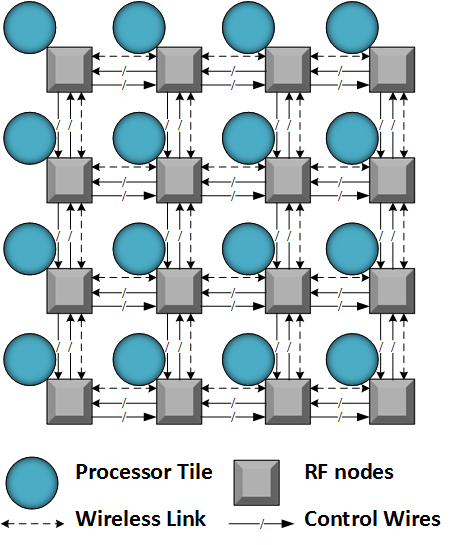
\includegraphics[scale=0.5]{Fig_4531729.png}
\caption{The Universe}
\label{fig:Fig_4531729}
\end{figure}

Suk-Bok Lee et al. in \citep{lee2009scalable}, propose a two-tiers hybrid wireless/wired architecture to interconnect hundreds to thousands of cores in chips multi-processor (CMP) using Sub-THz. This architecture benefits from the baseline 2-D concentrated mesh (Cmesh), which is basically a 2D-mesh that concentrate four cores or four L2 cache connected to one router, it provides a base network with very short wires and exploits a wireless backbone to enhance connectivity, reducing network latency. The network has two types of routers, viz. base routers, that make up the baseline Cmesh, and wireless routers, that have wireless interfaces to form a wireless backbone. The Sub-THz wireless infrastructure is a recursive structure called the Wcube that features a single transmit antenna and multiple receiver antennas at each micro wireless router and offers scalable performance in terms of latency and connectivity. Figure \ref{fig:Fig_lee2009scalable} illustrates a Wcube structure. This design provides from 20 to 45\% latency reduction, but it has to pay a price in power consumption that is comparable than current 2D wire line mesh design for a 1024-core systems.


\begin{figure}[ht]
\centering
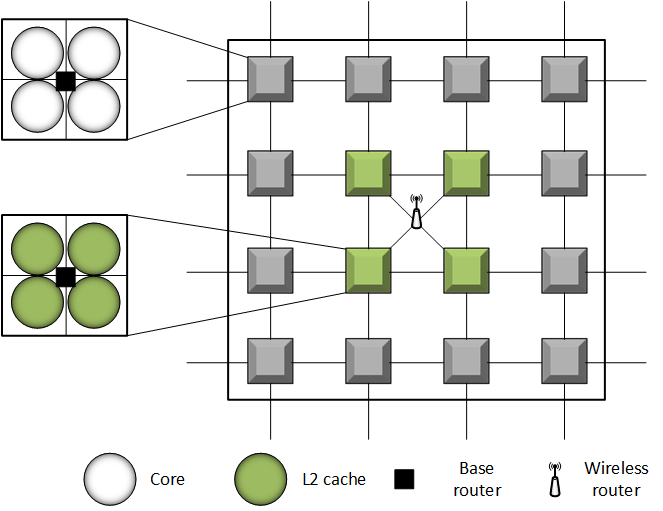
\includegraphics[scale=0.5]{Fig_lee2009scalable.png}
\caption{The Universe}
\label{fig:Fig_lee2009scalable}
\end{figure}

An inter-router wireless scalable express channel in the mm-wave frequency range for NoC architectures, called iWISE (inter-router Wireless Scalable Express channel), was proposed by Dominic DiTomaso et al. in \citep{6041529} that minimizes the power consumption via hybrid wireless communication channels, reduces the area overhead with smaller routers and shared buffers, and improves performance by minimizing the hop count. In this architecture the cores are arranged in a grid fashion and a wired mesh is used to connect adjacent routers and wireless links are connected between every router. These wireless links are shared such that every set can communicate with every other set including itself. Figure \ref{fig:Fig_6041529}a, illustrates an architecture called iWISE-64 (inter-router Wireless Scalable Express channel for 64 cores). Figure \ref{fig:Fig_6041529}b shows the logical organization of the cluster and sets for iWISE-64. Individual cluster are addressed by the notation C(c,s,g), where c is an arbitrary cluster numbered 0 up to C-1, s is a set numbered 0 up to S-1 and g is a group from 0 up to G-1. In iWISE-64 g is 0 because only need one group for 64 cores. This architecture is demonstrated to achieve a 2.5X in performance compared to other architectures like Wcube \citep{lee2009scalable}. iWISE-64 saves an average of approximately 20\% power over wireless networks and an average of 43\% power over all other electrical networks. In area overhead it saves over 10\% compared to a concentrated mesh (Cmesh) and approximately 40\% of total area compared to baseline wired mesh.

\begin{figure}[ht!]
\centering
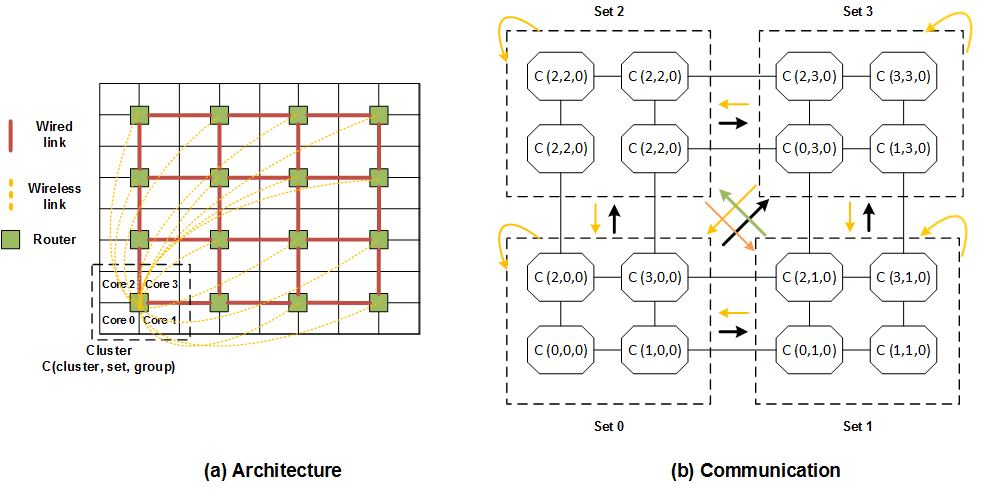
\includegraphics[scale=0.5]{Fig_6041529.png}
\caption{The Universe}
\label{fig:Fig_6041529}
\end{figure}



\section{Wireless Interface (WI)}


In WI, there are two main components, the antenna and the transceiver. According to the ITRS, the cut-off frequency and unity maximum available power gain frequency targets are 600 GHz and 1 THz respectively in 16 nm CMOS technology. With such scaling the required antenna and circuit areas will scale down allowing easy on-chip integration. One constraint in a WiNoC is that on-chip antenna provide the best power gain for the smallest area overhead. A metal zig-zag antenna has been demonstrated to possess these characteristics and suits this application. This antenna was used by Sujay Deb et al. in \citep{5540799} to design a millimeter (mm)-wave Wireless NoC, and it has demonstrated a good performance with a 3 dB bandwidth of 16 GHz with a center frequency of 62,5 GHz using 0,38 mm long zig-zag antenna. Another type of antenna that we can find in literature is a dipole antenna used in intra-chip UWB interconnection proposed by D. Zhao and Yin Wang in \citep{4531729}. This antenna has been implemented for 1 mm range data transmission at antenna length of 2,98 mm. Despite a reduction in antenna size by more than 20x, the current practice of integrating an antenna directly on silicon will cause a significant energy loss in a conductive silicon substrate. In order to minimizes the substrate loss, Suk-Bok Lee et al. in \citep {lee2009scalable} propose that an on-chip antenna should be placed in a polyimide layer (a few mils thick), which deposits on the top of top the top silicon, such that most electromagnetic energy can be confined within this low-loss dielectric layer. Simulations demonstrated that even though radiation attenuates significantly at the receive antenna (about -40dB at 1 cm away from transmitter), the receiver still has enough sensitivity to detect the signal.
To ensure the high throughput and energy efficiency of the WiNoC, the transceiver circuitry has to provide a very wide bandwidth as well as low power consumption. In designing on-chip wireless transceiver, low power design considerations need to be taken into account both at the architecture and circuit level. In a first approach we can try to use a classical coherent architecture with complex modulated signals (BPSK, QPSK, 16-QAM, FSK) and high spectral efficiency. However, such systems exhibit a low energy efficiency resulting in high power consumption that makes them unsuitable for battery powered devices. Kenichi Okada et al. in \citep {6339016} show in their work different modulations implemented in CMOS transceivers for inter-board communication and OOK modulation demonstrate a good performance in energy efficiency compared with the others because it allows a relatively simple circuit implementation. In literature most transceivers use OOK modulation for the reasons given above. Vincenzo Catania et al. in \citep{7459514} present a  generic WiNoC single channel OOK transceiver, illustrated in Figure \ref{fig:Fig_transceiverOOK3}, constituted by a transmitter and receiver which share the same antenna by means of a RF-switch. The main task of transmitters consists in adapting the data incoming from the electrical medium to the wireless medium by means of an antenna. In particular, a transmitter is constituted by a serializer which converts parallel streams of data (flits) in a serial fashion; a modulator which adapts a low frequency signal into a high frequency one; a power amplifier (PA) directly connected to the antenna which delivers the required transmitting power. It also comprises a token flow controller to decode incoming information and manage the token flow mechanism. In order to share the wireless medium among radio-hubs. Conversely, the receiver presents a Low Noise Amplifier (LNA) which amplifies incoming signals introducing less noise as possible; a demodulator which shifts high frequency signals into the baseband; a baseband amplifier and a Pulse Shaping filter that amplify and shape signals to obtain a digital signal which is stored in a specific buffer. 

\begin{figure}[ht!]
\centering
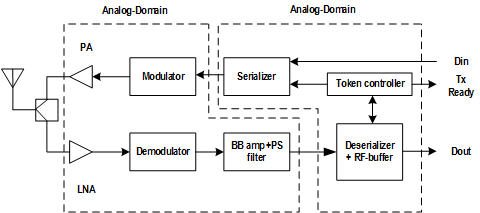
\includegraphics[scale=0.9]{transceiverOOK3.png}
\caption{The Universe}
\label{fig:Fig_transceiverOOK3}
\end{figure}

Sujay Deb et al. in \citep{6302124} propose another architecture for the transceiver, illustrated in Figure \ref{fig:Fig_transceiverOOK}. This architecture has some differences compared with the one given above. Firstly, the transmitter and receiver have their own antenna; secondly, an injection-lock voltage-controlled oscillator (VCO) is reused for TX and RX. Joined to the fact that the receiver uses a direct-conversion topology, a power-hungry phase-lock loop (PLL) is eliminated. Finally, a third difference is that it has pulse shaping filters in both TX and RX.



\begin{figure}[ht!]
\centering
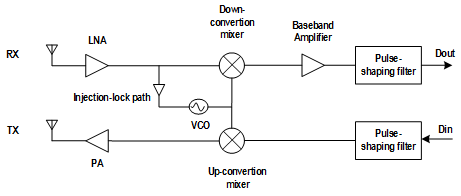
\includegraphics[scale=0.9]{transceiverOOK.png}
\caption{The Universe}
\label{fig:Fig_transceiverOOK}
\end{figure}



The transceivers given above, both works in mm-wave. Suk-Bok Lee et al. in \citep{lee2009scalable} propose another low power transceiver to work in a sub-Terahertz (100 - 500 GHz) on-chip wireless network. They show that a simple asynchronous Amplitude-Shift-Keying (ASK) system suffices to satisfy these requirements. Figure \ref{fig:Fig_transceiverOOK2} illustrates such a simple on-chip radio architecture, which has one oscillator and one ASK modulator in a TX and one demodulator and simple baseband circuit in RX.  


\begin{figure}[ht!]
\centering
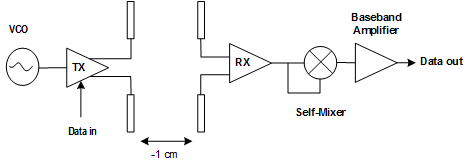
\includegraphics[scale=0.9]{transceiverOOK2.png}
\caption{The Universe}
\label{fig:Fig_transceiverOOK2}
\end{figure}

Finally, in literature there is a transceiver proposed by Alexandre Brière et al. in \citep{2015} that use BPSK modulation. It is doted of a medium access scheme based on orthogonal frequency division multiple access (OFDMA) to add the possibility for multiple senders to simultaneously use the same bandwidth. This transceiver uses a waveguide to allow inter cluster communication but it could be used in wireless communication due to the possibility of tuning Carbon Nano Tube (CNT) antennas to various frequencies that makes possible to communicate using Orthogonal Frequency Division Multiplexing (OFMD). However, challenges of fabrication and integration of CNT antennas with CMOS process may hinder its adoption in the near future. Another issue could be the surface that is mainly occupied by FFT/IFFT used in OFDM.


\section{Media Access Control}

In order to achieve the desired performance benefits using WiNoC, the available communication resources should be utilized optimally. Efficient media access mechanism is crucial for efficient utilization of the wireless channels. In this part, we will discuss about the different media access control (MAC) mechanisms used for WiNoCs.
A suitable MAC mechanism is very important to sustain an acceptable performance level. The adopted MAC has to be simple and lightweight. It should not introduce undue area and power overheads. Implementation of the MAC protocol also depends on that characteristics of physical layer. Due to the limitations in the available bandwidth and complexity of transceivers designs, multiple non-overlapping channels at high operating frequencies is a non-scalable solution. 
MAC protocols can be classifying in three broad classes: Channel Partitioning (CP), Random Access (RA), Taking Turns (TT). The CP divides into smaller “pieces”, either into time slots, frequency or code. In RA, the channel is not divided and allow collisions. And finally, In TT each node takes turns to dispatch information, but nodes with more to send can take longer turns.
In literature, we can find WiNoCs within each class. For example, The Token Passing Multiple Access (TPMA) belongs to TT. This schema is a common adopted scheme for Wireless Network-on-Chip (WiNoC). TPMA uses a token to authorize nodes rights to access the wireless media. The key issue of toking passing protocol is how to pass the token. The most popular passing mechanism uses a round-robin manner which is a max-min fair scheduling scheme.
Vincenzo Catania et al. adopted this schema in their work \citep{7459514}. They used a 256-node NoC in which 4 and 16 radio-hubs are used for implementing wireless long-rang communications, respectively. The 16x16 mesh topology is partitioned into a number of regular regions depending on the number of radio-hubs. The simulations show that for a low packet injection rate (pir) values WiNoC-16 and WinoC-4 are quite similar, whereas as the pir increases WiNoC-4 exhibits lower communication delay than WiNoC-16. To explain this behavior, it should be recalled that having more radio-hubs implies having longer token round time. 
Dominic DiTomaso et al. in \citep{6041529} use the same schema but the hierarchical architecture, proposed in their work allow to use a token with different bit size one by each transceiver used in its group and set, in addition each antenna used is omnidirectional, therefore it could manage four communications at the same time with this token passing  protocol. The TPAM is used with different architectures and different amounts of cores, with 16 cores \citep{7459513}, 256 cores (\citep{7459514}, \citep{6041529})  and 512 cores (\citep {6302124}, \citep {5540799}, \citep {5551123}). While the amounts of cores increase the latency increase too. Hence, the token passing protocol does not scale well with increasing number of wireless nodes. To overcome this issue, it is possible to implement a channel partitioning (CP) protocol like CDMA or FMDA.  Using multiple access mechanism such as code division multiple access (CDMA) the number of simultaneous access can be increased. Consequently, this will improve the performance of WiNoCs links significantly. Anuroop Vidapalapati et al. in \citep{6272112} use a Walsh-Hadamard code of eight CDMA chips per bit, which enables seven simultaneous transmissions using the wireless medium. The proposed architecture contains 64 and 128 cores and the simulations show that CDMA is capable of improving the performance compared to previous work with token passing multiple access (TPMA) with the same architecture.
Suk-Book Lee et al. in \citep{lee2009scalable} uses Frequency Division Multiple Access (FDMA) with sub terahertz WiNoC. This architecture uses different frequency channel to deliver a packet at each wireless router. Each router has one transmitter, as well as 2n receivers each of which tunes to a different frequency channel. 
A Random Access (RA) protocol like Carrier Sense Multiple Access (CSMA) is discussed in \citep{7062254} to be implemented in wireless interconnects NoC. This protocol was compared with a TPMA-based architecture using 16 and 64 cores. Simulations shows that CSMA have higher upper bound of throughput than TPMA. This could increase the channel utilization and could enhance the throughput.


\medskip

%Sets the bibliography style to UNSRT and imports the 
%bibliography file "samples.bib".
\bibliographystyle{plain}
\bibliography{references}
\end{document}
